\chapter{TTL and multiplexer}
In this session we first measured the latency between the input and output signal of a 74LS00, then we used a NOT gate with open collector to turn on and off a LED, thirdly we designed and built an half dulpex with two 3state gates and lastly we designed and implemented a multiplexer with 4 signals and two bit of selection.

\section{Materials}
\begin{itemize}
\item A resistor
\item A LED
\item Power supply RIGOL DP831A
\item Waveform generator RIGOL DG1032
\item Multimeter RIGOL DM3068
\item 74LS00
\item 74LS05
\item 74LS04
\item 74LS125
\end{itemize}

\section{Experimental setup}
In order to measure the time propagation of the signal in the 7400 gate we used the configuration in figure \ref{latency}. As input we used a square wave with 0-5 V voltage and a 100 kHz frequency.
\begin{figure}[H]
\centering
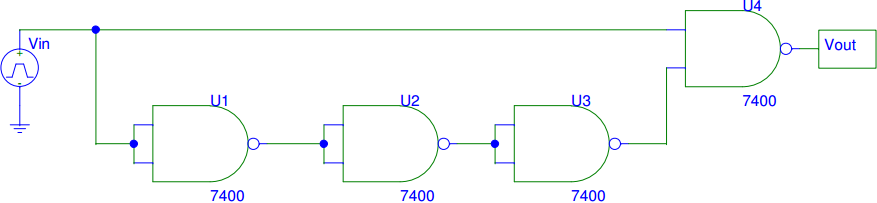
\includegraphics[width=.7\textwidth]{10/latency.png}
\caption{The circuit used for measuring the latency in the propagation of a digital input}\label{latency}
\end{figure}
The NOT gate test was acheved implementing a circuit for switching on and off a LED. The circuit is in figure \ref{LED_ON_OFF} and has a power supply of 9 V: since the voltage drop in the LED and the gate is 1.4 V in total and we must have a 5 mA current flowing, this meant that we needed a pull-up resistor of approximately 1.5 k$\Omega$.
\begin{figure}[H]
\centering
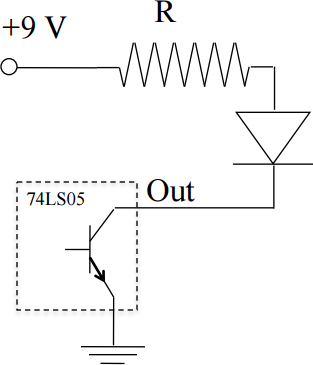
\includegraphics[width=.3\textwidth]{10/LED_ON_OFF.png}
\caption{NOT TTL Open Collector}\label{LED_ON_OFF}
\end{figure}
we built the half duplex as in figure \ref{TTL_3state}. We chose two signals to be transmitted and put each one as the input of a 3-state: the first was a square wave and the other just the ground voltage. We than used an enabling signal to select which of the two had to be transmitted: we connected this directly to the enable pin of a 3-state gate and negated to the same pin of the other gate. We then just put toghether the two gates output and connected them to a LED in order to verify the correct circuit working: actually just one signal passed at any time.
\begin{figure}[H]
\centering
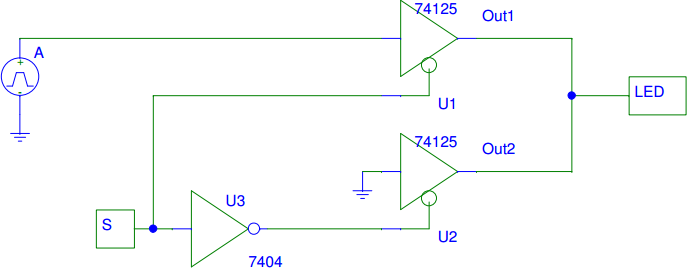
\includegraphics[width=.7\textwidth]{10/TTL_3state.png}
\caption{Half duplex used for sharing a transmission channel}\label{TTL_3state}
\end{figure}
Lastly we designed a mutiplexer to transmit 4 different signals to another group using again just one wire (plus one for the ground and two for the selection). First we needed to design a 2 bits selector to choose only one among the 4 signals: this was implemented with the circuit in figure \ref{multi_select}.
\begin{figure}[H]
\centering
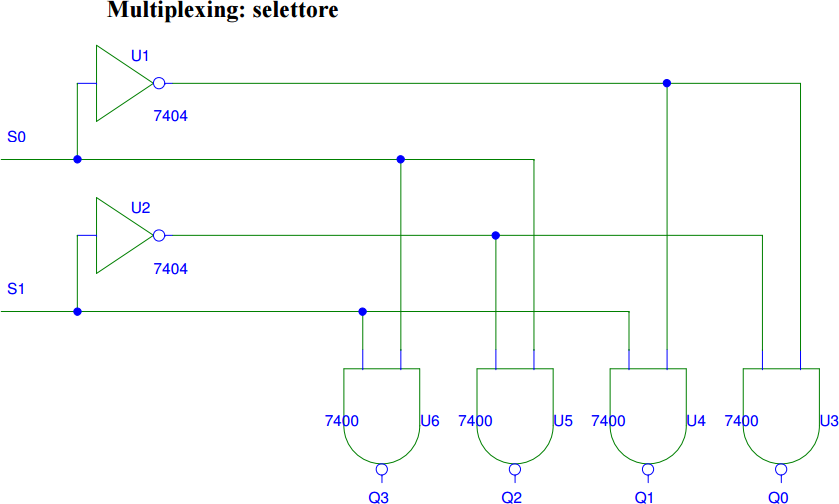
\includegraphics[width=.7\textwidth]{10/multi_select.png}
\caption{The selection circuit: the choice of the enabled channel is made with the 2 bits S0 and S1}\label{multi_select}
\end{figure}
Then we used each signal from the selector to enable 4 different 3-state gates, which inputs were our channels D0,D1,D2,D3 with the informations to be transmitted. The 4 outputs had then been put together to be transmitted through only one wire, like we did in the half duplex. This part is shown in figure \ref{multi_wired}.
\begin{figure}[H]
\centering
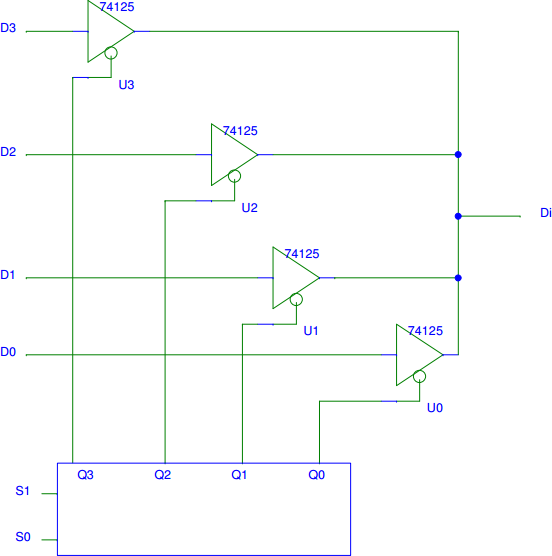
\includegraphics[width=.7\textwidth]{10/multi_wired.png}
\caption{The signal from the selector used for blocking and allowing the chosen channel}\label{multi_wired}
\end{figure}
\begin{table}[H]
\centering
\begin{tabular}{c|c|c}
 S0 & S1 & Channel enabled\\
 \hline
 0 & 0   & D0\\
 0 &1    &  D1\\
 1&0    & D2\\ 
 1 &1    &  D3\\ 
\end{tabular}\caption{2 bits selector logic}
\end{table}
We then used a cable to pass to our friends of another group the 3 wires needed for the informations decoding (one with the informations and two for the selection): they were that way able to know which channel was transmitting. The common reference used by the 2 group had to be the same, so we used the earth voltage of the building and successfully trasmitted various signal to the other side of the room. 

\section{Data analysis}
From the graph \ref{latency_plot} we can evaluate the time delay caused by a single gate. We see that the signal took about $14.40 \pm 0.08$ ns from when it started descending to when it started rising, time that divided by the three gates gives $4.800 \pm 0.027$ ns per gate: this is an average of the high-to-low ropagation delay and the low-to-high one.\\
We chose only the part of the signal with a negative derivative because that is the period during which the three gates changes their state.
\begin{figure}[H]
\centering
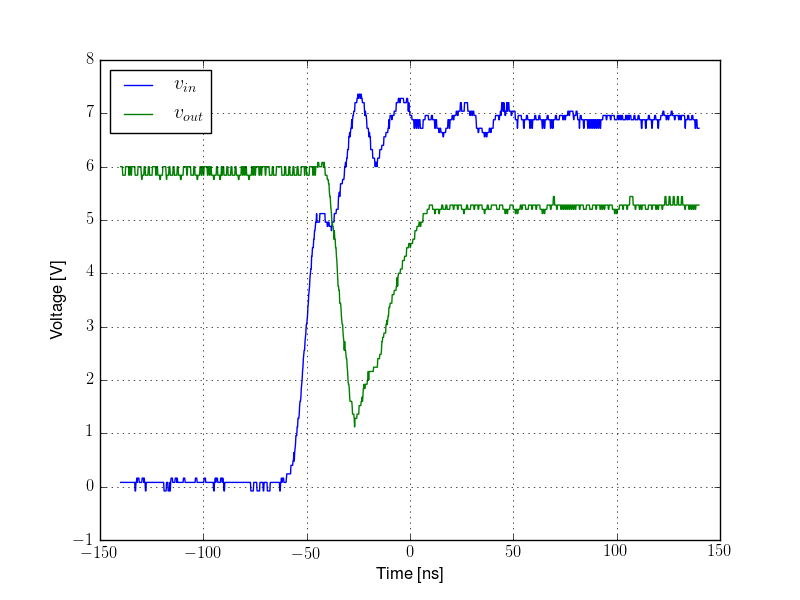
\includegraphics[width=.7\textwidth]{10/latency_plot.png}
\caption{The plot shows the delay caused by the propagation of the signal in 3 gates}\label{latency_plot}
\end{figure}
